\documentclass[12pt,a4paper]{article}

% ─── Page Layout ───────────────────────────────────────────────────────────────
\usepackage[a4paper, margin=0.8in, headheight=14pt]{geometry}

% ─── Fonts (XeLaTeX) ───────────────────────────────────────────────────────────
\usepackage{fontspec}
\usepackage{unicode-math}
\setmainfont{TeX Gyre Pagella}
\setmonofont[Scale=0.88]{TeX Gyre Cursor}
\setmathfont{Latin Modern Math}

% ─── Packages ──────────────────────────────────────────────────────────────────
\usepackage{xcolor}
\usepackage{colortbl}
\usepackage{titlesec}
\usepackage{enumitem}
\usepackage{tabularx}
\usepackage{booktabs}
\usepackage{array}
\usepackage{amsmath}
\usepackage{tikz}
\usetikzlibrary{shapes.geometric, arrows.meta, positioning, calc, fit, decorations.pathreplacing}
\usepackage{tcolorbox}
\tcbuselibrary{skins, breakable}
\usepackage{hyperref}
\usepackage{fancyhdr}
\usepackage{graphicx}
\usepackage{microtype}
\hyphenpenalty=10000
\exhyphenpenalty=10000
\sloppy
\usepackage{caption}
\usepackage{setspace}
\usepackage{multirow}
\usepackage{tocloft}

% ─── Q&A helper ────────────────────────────────────────────────────────────────
\newcommand{\Q}[1]{\textbf{#1}\par\noindent\ignorespaces}

% ─── Colour Palette ────────────────────────────────────────────────────────────
\definecolor{myred}{RGB}{196,30,58}
\definecolor{mydark}{RGB}{30,30,50}
\definecolor{mygreen}{RGB}{14,120,80}
\definecolor{myteal}{RGB}{0,130,140}
\definecolor{myamber}{RGB}{180,100,0}
\definecolor{mypurple}{RGB}{100,30,160}
\definecolor{mygray}{RGB}{246,247,249}
\definecolor{mgframe}{RGB}{180,185,200}
\definecolor{watermark}{RGB}{145,150,170}
\definecolor{hdrred}{RGB}{250,232,235}
\definecolor{hdrgreen}{RGB}{220,244,233}
\definecolor{hdrteal}{RGB}{220,242,244}
\definecolor{hdramber}{RGB}{253,242,215}
\definecolor{hdrpurple}{RGB}{238,228,255}
\definecolor{hdrgray}{RGB}{238,240,245}
\definecolor{rowalt}{RGB}{250,251,253}

% ─── Section Formatting ────────────────────────────────────────────────────────
\titleformat{\section}
  {\large\bfseries\color{myred}}{\thesection.}{0.5em}{}
  [\vspace{1pt}{\color{myred}\rule{\linewidth}{0.8pt}}]
\titleformat{\subsection}
  {\normalsize\bfseries\color{myteal}}{\thesubsection}{0.5em}{}
\titlespacing*{\section}{0pt}{18pt}{7pt}
\titlespacing*{\subsection}{0pt}{11pt}{4pt}

% ─── Paragraph ─────────────────────────────────────────────────────────────────
\setlength{\parindent}{0pt}
\setlength{\parskip}{4pt}

% ─── TOC Styling ───────────────────────────────────────────────────────────────
\renewcommand{\cfttoctitlefont}{\large\bfseries\color{myred}}
\renewcommand{\cftaftertoctitle}{\par\noindent{\color{myred}\rule{\linewidth}{0.8pt}}}
\setlength{\cftbeforetoctitleskip}{0pt}
\setlength{\cftaftertoctitleskip}{6pt}
\renewcommand{\cftsecfont}{\normalsize\bfseries\color{mydark}}
\renewcommand{\cftsecpagefont}{\normalsize\bfseries\color{mydark}}
\renewcommand{\cftsecleader}{\cftdotfill{\cftdotsep}}
\setlength{\cftbeforesecskip}{7pt}
\renewcommand{\cftsubsecfont}{\small\color{mydark}}
\renewcommand{\cftsubsecpagefont}{\small\color{mydark}}
\setlength{\cftbeforesubsecskip}{3pt}
\setlength{\cftsubsecindent}{1.4em}

% ─── Table helpers ─────────────────────────────────────────────────────────────
\renewcommand{\arraystretch}{1.45}
\setlength{\tabcolsep}{6pt}
\arrayrulecolor{mydark}
\newcolumntype{B}[1]{>{\small\bfseries\raggedright\arraybackslash}m{#1}}
\newcolumntype{Y}{>{\small\raggedright\arraybackslash}X}
\renewcommand{\tabularxcolumn}[1]{m{#1}}

% ─── Header / Footer ───────────────────────────────────────────────────────────
\pagestyle{fancy}
\fancyhf{}
\fancyhead[L]{\small\color{myred}\textbf{PE-EC603A}\;\color{mydark}--- Introduction to MEMS}
\fancyhead[R]{\small\color{myteal}\textbf{Module 1 Notes}}
\fancyfoot[C]{\small\color{mydark}\thepage}
\fancyfoot[R]{\small\color{watermark}\textit{\copyright\ Biraj}}
\renewcommand{\headrulewidth}{0.5pt}
\renewcommand{\footrulewidth}{0.3pt}

% ─── Hyperref ──────────────────────────────────────────────────────────────────
\hypersetup{
  colorlinks=true, linkcolor=myteal, urlcolor=myteal,
  pdfauthor={Biraj Sarkar},
  pdftitle={PE-EC603A --- Module 1 Notes}
}

% ─── tcolorbox styles ──────────────────────────────────────────────────────────
\tcbset{
  tikzbox/.style={
    colback=mygray, colframe=mgframe, boxrule=0.6pt, arc=4pt,
    left=8pt, right=8pt, top=6pt, bottom=6pt,
    colbacktitle=mgframe, coltitle=mydark,
    fonttitle=\small\bfseries
  },
  defbox/.style={
    colback=hdrgreen, colframe=mygreen, boxrule=0.8pt, arc=4pt,
    left=9pt, right=9pt, top=6pt, bottom=6pt,
    colbacktitle=mygreen, coltitle=white,
    fonttitle=\small\bfseries
  },
  formulabox/.style={
    colback=hdrteal, colframe=myteal, boxrule=0.8pt, arc=4pt,
    left=9pt, right=9pt, top=7pt, bottom=7pt,
    colbacktitle=myteal, coltitle=white,
    fonttitle=\small\bfseries
  },
  examplebox/.style={
    colback=hdramber, colframe=myamber, boxrule=0.8pt, arc=4pt,
    left=9pt, right=9pt, top=6pt, bottom=6pt,
    colbacktitle=myamber, coltitle=white,
    fonttitle=\small\bfseries
  },
  masonbox/.style={
    colback=hdrpurple, colframe=mypurple, boxrule=0.8pt, arc=4pt,
    left=9pt, right=9pt, top=6pt, bottom=6pt,
    colbacktitle=mypurple, coltitle=white,
    fonttitle=\small\bfseries
  },
  exambox/.style={
    colback=hdrpurple, colframe=mypurple, boxrule=1pt, arc=5pt,
    left=10pt, right=10pt, top=8pt, bottom=8pt,
    colbacktitle=mypurple, coltitle=white,
    fonttitle=\bfseries,
    breakable, title after break={\textbf{Frequently Asked / Viva Questions (contd.)}}}
}
% Make all boxes breakable across pages
\tcbset{breakable}

% ─── TikZ styles ───────────────────────────────────────────────────────────────
\tikzset{
  block/.style={rectangle, draw=myteal, fill=hdrteal,
    text width=2.4cm, align=center, minimum height=0.95cm,
    font=\small, rounded corners=3pt, line width=0.7pt},
  redblock/.style={rectangle, draw=myred, fill=hdrred,
    text width=2.4cm, align=center, minimum height=0.95cm,
    font=\small, rounded corners=3pt, line width=0.7pt},
  netnode/.style={rectangle, draw=myteal, fill=hdrteal,
    text width=1.5cm, align=center, minimum height=0.8cm,
    font=\small, rounded corners=3pt, line width=0.7pt},
  sumjunc/.style={circle, draw=myamber, fill=hdramber,
    minimum size=0.62cm, font=\small, line width=0.8pt},
  snode/.style={circle, draw=mypurple, fill=hdrpurple,
    minimum size=0.55cm, font=\footnotesize, line width=0.7pt},
  arrow/.style={-Stealth, thick, color=mydark},
  redarrow/.style={-Stealth, thick, color=myred},
  line/.style={thick, color=mydark}
}

% ═══════════════════════════════════════════════════════════════════════════════
\begin{document}
% ═══════════════════════════════════════════════════════════════════════════════

\begin{center}
  {\LARGE\bfseries\color{myred} PE-EC603A --- Introduction to MEMS}\\[5pt]
  {\normalsize\color{mydark} Semester VI \quad$\bullet$\quad 3L:0T:0P \quad$\bullet$\quad 3 Credits}\\[3pt]
  {\normalsize\color{myteal}\textbf{Module 1 Exam Notes: Introduction and Historical Background}}\\[3pt]
  {\small\color{mydark} CGEC \;$|$\; B.Tech ECE (2023--27) \;$|$\; \textit{Biraj Sarkar}}
\end{center}
\vspace{2pt}
\noindent{\color{myred}\rule{\linewidth}{1.5pt}}
\vspace{2pt}

\hypersetup{linkcolor=mydark}
\tableofcontents
\hypersetup{linkcolor=myteal}
\newpage

% ===============================================================================
\section{Fundamentals of MEMS and Microsystems}
% ===============================================================================

Micro-Electro-Mechanical Systems (MEMS) represent a technology that combines mechanical elements, sensors, actuators, and electronics on a common silicon substrate through micro-fabrication technology.

\subsection{Definition and Concepts}
\begin{tcolorbox}[defbox]
\textbf{MEMS (Micro-Electro-Mechanical Systems):} An integrated micro-scale system combining electrical, mechanical, optical, chemical, or fluidic elements fabricated on a single chip using semiconductor manufacturing processes.
\end{tcolorbox}

\textbf{Core Characteristics of MEMS:}
\begin{itemize}[leftmargin=*, itemsep=3pt]
  \item \textbf{Scale:} Feature sizes typically range from 1 micrometer ($\mu$m) to 100 micrometers ($\mu$m), while the overall device footprint is usually between 20 $\mu$m and several millimeters.
  \item \textbf{Integration:} Merges high-precision micro-sensors (input), micro-actuators (output), and microelectronic circuitry (control/processing) on a monolithic silicon substrate.
  \item \textbf{Multi-physics:} Involves coupling across mechanical, electrical, thermal, magnetic, optical, fluidic, and chemical domains.
\end{itemize}

\subsection{Microsystems vs. Microelectronics}
While microelectronics deals with the processing and flow of electrical signals (electrons), microsystems interface directly with the physical environment by converting non-electrical physical variables into electrical signals, and vice versa.

\textbf{Structural Comparison:}\par\noindent
\begin{tabularx}{\linewidth}{|B{3.2cm}|Y|Y|}
\hline
\textbf{Feature} & \textbf{\color{myteal}Microelectronics (IC)} & \textbf{\color{mygreen}Microsystems (MEMS)} \\
\hline
\textbf{Primary Media} & Electrons and electrical signals. & Force, pressure, acceleration, chemical concentrations, heat, light, fluid flow. \\
\hline
\textbf{Components} & Transistors, diodes, resistors, capacitors (static elements). & Cantilevers, diaphragms, micro-valves, comb drives, micro-mirrors (moving parts). \\
\hline
\textbf{Packaging} & Standardized plastic/ceramic packages, sealed from environment. & Must expose the active sensor elements to the environment while shielding the electronics. \\
\hline
\textbf{Substrate} & Purely single-crystal silicon. & Silicon, glass, quartz, polymers (SU-8, PDMS), metals. \\
\hline
\textbf{Manufacturing} & Standard CMOS / planar processes. & CMOS + bulk/surface micromachining, wafer bonding, high-aspect-ratio lithography (LIGA). \\
\hline
\end{tabularx}

\subsection{Generalized MEMS System Architecture}
A complete microsystem acts as a bridge between the physical environment and the electronic processing domain. It typically contains five functional components:

\begin{tcolorbox}[tikzbox, title={Generalized MEMS System Control Loop}]
\centering
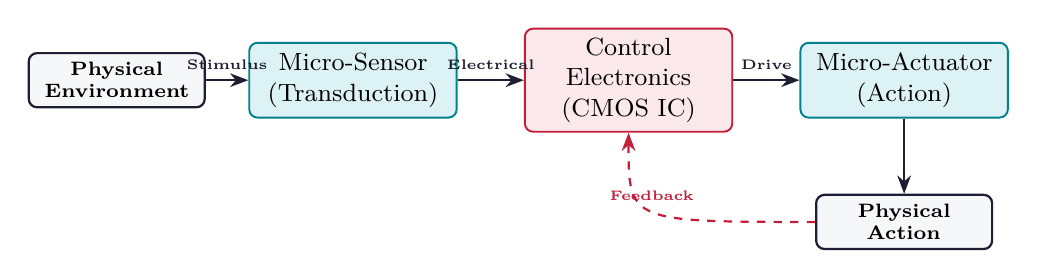
\begin{tikzpicture}[node distance=1.4cm, thick]
  % Nodes
  \node[rectangle, draw=mydark, fill=mygray, rounded corners=3pt, text width=2.0cm, align=center, font=\scriptsize\bfseries] (env) at (-5.0, 0) {Physical\\Environment};
  
  \node[block] (sensor) at (-2.0, 0) {Micro-Sensor\\(Transduction)};
  
  \node[rectangle, draw=myred, fill=hdrred, rounded corners=3pt, text width=2.4cm, align=center, minimum height=0.95cm, font=\small, line width=0.7pt] (control) at (1.5, 0) {Control\\Electronics\\(CMOS IC)};
  
  \node[block] (actuator) at (5.0, 0) {Micro-Actuator\\(Action)};
  
  \node[rectangle, draw=mydark, fill=mygray, rounded corners=3pt, text width=2.0cm, align=center, font=\scriptsize\bfseries] (action) at (5.0, -1.8) {Physical\\Action};

  % Connections
  \draw[arrow] (env) -- (sensor) node[midway, above, font=\tiny\bfseries] {Stimulus};
  \draw[arrow] (sensor) -- (control) node[midway, above, font=\tiny\bfseries] {Electrical};
  \draw[arrow] (control) -- (actuator) node[midway, above, font=\tiny\bfseries] {Drive};
  \draw[arrow] (actuator) -- (action);
  
  % Feedback loop
  \draw[redarrow, dashed] (action.west) .. controls (1.5, -1.8) .. (control.south) node[midway, above, font=\tiny\bfseries] {Feedback};
\end{tikzpicture}
\end{tcolorbox}

% ===============================================================================
\section{History and Milestones of Miniaturization}
% ===============================================================================

The evolution of MEMS spans several decades, transitioning from basic laboratory micro-mechanical discoveries to commercial monolithic consumer electronic devices.

\subsection{Richard Feynman's Vision (1959)}
The conceptual foundation of nanotechnology and micro-manufacturing was laid by physicist Richard Feynman on December 29, 1959, during his famous American Physical Society lecture at Caltech: \textit{"There's Plenty of Room at the Bottom"}.
\textbf{Key Concepts Proposed by Feynman:}
\begin{itemize}[leftmargin=*, itemsep=2.5pt]
  \item \textbf{Writing at Atomic Scale:} Suggested writing the entire 24 volumes of the Encyclopaedia Britannica on the head of a pin by scaling down the font size.
  \item \textbf{Micro-machining Tools:} Envisioned building micro-scale mechanical hands that could build even smaller machines, cascading down to build atomic-scale factories.
  \item \textbf{MEMS Actuators:} Proposed the creation of tiny motors (micro-motors) and electrostatic actuators using micro-lithographic techniques.
  \item \textbf{Physical Scaling:} Highlighted that as machines scale down, the relative importance of physical forces changes (gravity fades, while surface tension and electrostatic forces dominate).
\end{itemize}

\subsection{Key Historical Milestones}
The realization of Feynman's vision was enabled by the development of silicon semiconductor manufacturing and micromachining processes:
\begin{itemize}[leftmargin=*, itemsep=4pt]
  \item \textbf{1954 --- Discovery of Piezoresistivity in Silicon:} C. S. Smith discovered that silicon exhibits a large change in electrical resistance when mechanical stress is applied. This made silicon an exceptional material for pressure and strain sensors.
  \item \textbf{1967 --- Resonant Gate Transistor (RGT):} Developed by Harvey Nathanson at Westinghouse. It was the first batch-fabricated MEMS device, utilizing a moving gold cantilever beam acting as the gate element of a MOS transistor.
  \item \textbf{1970s --- Silicon Bulk Micromachining:} Techniques for anisotropic chemical etching of silicon (using KOH) were perfected, enabling the production of thin silicon membranes for pressure sensors.
  \item \textbf{1980s --- Surface Micromachining:} R. T. Howe and R. S. Muller at UC Berkeley developed surface micromachining. They used polysilicon as the structural material and silicon dioxide ($SiO_2$) as the sacrificial material to release free-moving mechanical structures like micro-cantilevers and gears.
  \item \textbf{1989 --- Electrostatic Comb Drive:} Developed by W. C. Tang, T. H. Nguyen, and R. T. Howe. It introduced lateral comb structures that generate electrostatic forces, forming the basis of micro-resonators and gyroscopes.
  \item \textbf{1990s --- Commercialization and DRIE:} The invention of Deep Reactive Ion Etching (DRIE) by the Bosch Process enabled etching of high-aspect-ratio trenches in silicon. Commercialization succeeded with ADI's ADXL50 accelerometer (for automotive airbag deployment) and TI's Digital Micromirror Device (DMD) for projectors.
\end{itemize}

% ===============================================================================
\section{Applications of MEMS}
% ===============================================================================

MEMS technology is ubiquitous across several key industrial sectors:

\subsection{Automotive Industry}
The automotive sector was the primary driver of MEMS commercialization, requiring high reliability and low-cost sensor components.
\begin{itemize}[leftmargin=*, itemsep=3pt]
  \item \textbf{Airbag Accelerometers:} Capable of measuring sudden deceleration ($50\text{ g}$ to $100\text{ g}$) to deploy airbags within milliseconds.
  \item \textbf{Electronic Stability Control (ESC):} Uses MEMS gyroscopes and accelerometers to measure vehicle yaw rate and lateral acceleration, applying differential braking to prevent skids.
  \item \textbf{Tire Pressure Monitoring Systems (TPMS):} Wireless piezoresistive pressure sensors mounted inside the tires to monitor inflation levels.
\end{itemize}

\subsection{Consumer Electronics}
MEMS enabled the miniaturization and touch interface revolution in personal devices.
\begin{itemize}[leftmargin=*, itemsep=3pt]
  \item \textbf{Smartphones:} Utilize 3-axis MEMS accelerometers (screen auto-rotation), gyroscopes (mobile gaming, stabilization), and MEMS barometers (altitude tracking).
  \item \textbf{MEMS Microphones:} Capacitive micro-scale microphones replacing traditional electret condenser microphones (ECM), offering better sound quality, thermal stability, and noise cancellation.
  \item \textbf{Display Systems (TI DMD):} Digital Micromirror Devices contain millions of microscopic electrostatic mirrors on a single chip, controling light reflections for digital cinema projectors.
\end{itemize}

\subsection{Medical and Biomedical (Bio-MEMS)}
The intersection of MEMS and biomedical engineering has created a new class of diagnostics and therapy.
\begin{itemize}[leftmargin=*, itemsep=3pt]
  \item \textbf{Disposable Pressure Sensors:} Piezoresistive catheter tip sensors used for real-time arterial blood pressure monitoring during surgeries.
  \item \textbf{Lab-on-a-Chip (LoC):} Microfluidic channels, pumps, and valves integrated on a chip to perform complex blood analysis and DNA profiling rapidly with microliters of sample.
  \item \textbf{Microneedles and Drug Delivery:} Array of silicon microneedles ($100\ \mu\text{m}$ to $500\ \mu\text{m}$ long) that penetrate the outer dead skin layer painlessly to deliver transdermal drug therapies.
\end{itemize}

\newpage
% ===============================================================================
% MANDATORY QUICK REVISION PAGE
% ===============================================================================
\begin{center}
  {\large\bfseries\color{myred} Quick Revision --- Module I}\\[3pt]
  {\small\color{mydark} Introduction and Historical Background $|$ PE-EC603A}
\end{center}
\noindent{\color{myred}\rule{\linewidth}{1.2pt}}
\vspace{4pt}

\begin{tcolorbox}[formulabox, title={\textbf{Key Concepts and Parameters}}]
\renewcommand{\arraystretch}{1.3}
\begin{tabularx}{\linewidth}{B{3.8cm} X}
Aspect Ratio (AR)        & $\text{Aspect Ratio} = \displaystyle\frac{\text{Height } (h)}{\text{Width } (w)}$ \\[8pt]
Feynman's Scaling Rule   & $F \propto L^n$ \quad (Forces scale down differently depending on $n$) \\[4pt]
Piezoresistive Effect    & $\displaystyle\frac{\Delta R}{R} = G \cdot \epsilon$ \quad ($G$ = Gauge Factor, $\epsilon$ = Mechanical Strain)
\end{tabularx}
\end{tcolorbox}

\begin{tcolorbox}[defbox, title={\textbf{One-Line Definitions}}]
\begin{itemize}[leftmargin=*, itemsep=2.5pt, topsep=0pt]
  \item \textbf{MEMS:} Micro-scale integrated systems combining mechanical, electrical, and control functions on a single silicon chip.
  \item \textbf{Microsystem:} An engineering system containing sensors, actuators, and electronics to bridge the physical and electrical domains.
  \item \textbf{Aspect Ratio:} The ratio of the height of a microfabricated structure to its lateral width.
  \item \textbf{Piezoresistivity:} The change in electrical resistivity of a material (especially silicon) under applied mechanical stress.
  \item \textbf{Sacrificial Layer:} A temporary film layer ($SiO_2$) deposited during surface micromachining, etched away later to release moving parts.
  \item \textbf{Structural Layer:} The functional, moving material layer (usually Polysilicon) that forms the core device structure in surface micromachining.
  \item \textbf{DRIE:} Deep Reactive Ion Etching, an anisotropic dry etching process used to fabricate high-aspect-ratio silicon trenches.
\end{itemize}
\end{tcolorbox}

\begin{tcolorbox}[exambox, title={\textbf{Frequently Asked / Viva Questions}}]
\begin{enumerate}[topsep=0pt, label=\textbf{Q\arabic*.}, itemsep=5pt]
  \item \Q{What is the primary difference between a sensor and an actuator in a MEMS device?}
    A sensor converts physical variables (e.g., pressure, acceleration) into electrical signals. An actuator converts electrical signals into physical motion or action (e.g., micro-mirror tilt, micro-valve opening).
  \item \Q{How did C. S. Smith's 1954 discovery of piezoresistivity influence MEMS technology?}
    Smith's discovery showed that silicon's resistance changes significantly under stress, forming the transduction basis for pressure sensors, accelerometers, and strain gauges.
  \item \Q{Why did Richard Feynman's 1959 speech serve as the conceptual basis for MEMS?}
    Feynman predicted that machines could be scaled down, that micro-machining could build micro-motors, and that physical scaling would shift dominance from gravity to electrostatic and surface forces.
  \item \Q{What is the structural role of a sacrificial layer in surface micromachining?}
    It acts as a temporary spacer supporting the structural layer during deposition. Once etched away (released) with an acid, it leaves the structural layer suspended and free to move.
  \item \Q{Why is single-crystal silicon the dominant substrate material in MEMS?}
    Silicon has excellent mechanical properties: no mechanical hysteresis, high fatigue strength, can be easily batch-fabricated using established CMOS semiconductor facilities.
  \item \Q{What was the Resonant Gate Transistor (RGT) and why was it a milestone?}
    Developed in 1967, it was the first batch-fabricated MEMS device. It used a moving gold cantilever as a transistor gate, proving mechanical elements could be integrated with microelectronics.
  \item \Q{Why is packaging more complex for MEMS devices compared to standard Integrated Circuits (ICs)?}
    ICs are hermetically sealed from the environment. MEMS sensors must interface directly with external media (like air or fluid) while simultaneously protecting sensitive control electronics.
  \item \Q{Explain the function of a MEMS gyroscope in consumer electronics.}
    It measures the angular rate of rotation (yaw, pitch, roll), enabling camera image stabilization, vehicular electronic stability control, and smartphone motion controls.
  \item \Q{What is LIGA technology and when is it preferred?}
    LIGA is a German acronym for lithography, electroplating, and molding. It uses high-energy X-ray lithography to fabricate structures with extremely high aspect ratios.
  \item \Q{State two applications of Bio-MEMS.}
    Disposable catheter tip blood pressure sensors and Lab-on-a-Chip (LoC) microsystems for rapid blood diagnosis and DNA sequencing.
  \item \Q{How does a MEMS accelerometer in an automotive airbag sensor function?}
    A suspended proof mass deflects under sudden deceleration, changing the capacitance between moving and fixed electrodes to trigger the airbag within milliseconds.
\end{enumerate}
\end{tcolorbox}

\begin{tcolorbox}[tikzbox, title={Comparison: Silicon (MEMS) vs. Steel (Macro-engineering)}]
\renewcommand{\arraystretch}{1.45}
\par\noindent
\begin{tabularx}{\linewidth}{|B{3.2cm}|Y|Y|}
\hline
\textbf{Property} & \textbf{\color{myteal}Silicon (Si)} & \textbf{\color{myamber}Structural Steel} \\
\hline
\textbf{Yield Strength} & $7\text{ GPa}$ (higher than steel). & $0.2 - 0.5\text{ GPa}$. \\
\hline
\textbf{Young's Modulus} & $190\text{ GPa}$ (stiff, similar to steel). & $200\text{ GPa}$. \\
\hline
\textbf{Mechanical Hysteresis} & Negligible (extremely elastic). & Significant (plastic deformation). \\
\hline
\textbf{Fatigue Lifetime} & Infinite (no dislocation movement under stress). & Finite (dislocations accumulate, causing fracture). \\
\hline
\textbf{Density} & $2.3\text{ g/cm}^3$ (lightweight). & $7.8\text{ g/cm}^3$. \\
\hline
\end{tabularx}
\end{tcolorbox}

\end{document}
